\section{Logical Computations with Neurons}
The neurophysiologist Warren McCulloch and the mathematician Walter Pitts proposed, in 1943, a very simple model of the biological neuron, which became known as artificial neuron. It has one or more binary inputs and one binary output. The artificial neuron activates its output when more than a certain number of its inputs are active. 

Let's see what these networks do:
\begin{itemize}
    \item The network \ref{ANNs1} says: if neuron A is activated, then neuron C gets activated as well since it receives two input signals from neuron A. on the contrary if A is off, C is off as well.
    \item The network \ref{ANNs2} performs a logical \textit{AND}. Neuron C is activated only when both neurons A and B are activated. 
    \item The network \ref{ANNs3} performs a logical \textit{OR}. Neuron C gets activated if either neuron A or B is activated. Or both. 
    \item The network \ref{ANNs4} performs a complex logical proposition. Neuron C is activated only if neuron A is active and neuron B is off. They must follow this schema, otherwise, neuron C won't be activated. 
\end{itemize}

\begin{figure*}[t!]
    \centering
    \begin{subfigure}[b]{0.2\linewidth}
        \centering
        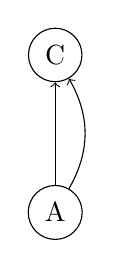
\begin{tikzpicture}[node distance=2cm]
                % First ANN
                \node[draw, circle] (A) at (0,0) {A};
                \node[draw, circle] (C) at (0,2) {C};
                
                \draw [->] (A) -- (C);
                \draw [->, bend right] (A) to (C);
            \end{tikzpicture}
            \caption{C=A}
            \label{ANNs1}
    \end{subfigure} \hfill
    \begin{subfigure}[b]{0.2\linewidth}
        \centering
       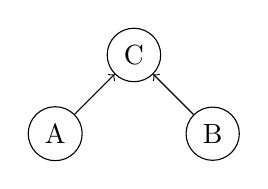
\begin{tikzpicture}[node distance=2cm]
            % Second ANN
            \node[draw, circle] (A) at (0, 0) {A}; 
            \node[draw, circle] (B) at (2, 0) {B}; 
            \node[draw, circle] (C) at (1, 1) {C}; 
            
            \draw [->] (A) -- (C);
            \draw [->] (B) -- (C);
        \end{tikzpicture}
        \caption{C = A $\land$ B}
        \label{ANNs2}
    \end{subfigure} \hfill
    \begin{subfigure}[b]{0.35\linewidth}
        \centering
        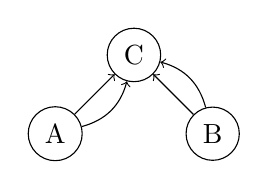
\begin{tikzpicture}[node distance=2cm]
            % Third ANN
            \node[draw, circle] (A) at (0, 0) {A};
            \node[draw, circle] (B) at (2, 0) {B};
            \node[draw, circle] (C) at (1, 1) {C};
            
            \draw [->] (A) -- (C);
            \draw [->, bend right] (A) to (C);
            \draw [->] (B) -- (C);
            \draw [->, bend right] (B) to (C);
        \end{tikzpicture}
        \caption{C = A $\lor$ B}
        \label{ANNs3}
    \end{subfigure} 
    \begin{subfigure}[b]{0.2\linewidth}
        \centering
        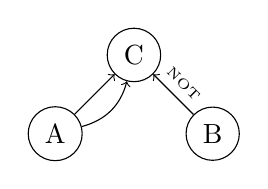
\begin{tikzpicture}[node distance=2cm]
            % Fourth ANN
            \node[draw, circle] (A) at (0, 0) {A};
            \node[draw, circle] (B) at (2, 0) {B};
            \node[draw, circle] (C) at (1, 1) {C};

            \draw [->] (A) -- (C);
            \draw [->, bend right] (A) to (C);
            \draw [->] (B) -- node[above, font=\tiny, sloped] {NOT} (C);
            
        \end{tikzpicture}
        \caption{C=A $\land \lnot$ B}
        \label{ANNs4}
    \end{subfigure}
    \caption{Artificial Neural Networks (ANNs) Performing Logical Computations - ANNs use multiple layers of neurons to perform logical computations.}
\end{figure*}
